\section*{Séquence symbolique}

Cette partie a été adaptée de \cite{3}.

\subsection*{Partitions}

Soit $(\Omega,\mathcal{B},\mu)$ un espace mesuré, i.e $\Omega$ est un ensemble non-vide appelé l'espace des états, $\mathcal{B}$ est une tribu de sous-ensembles de $\Omega$, et $\mu$ est une mesure positive sur l'espace mesurable $(\Omega,\mathcal{B})$. Une partition de $\Omega$ est une famille disjointe d'éléments de $\mathcal{B}$, non-vides et dont l'union est $\Omega$.
On suppose que $\mu(\Omega) \geq\infty$, on peut alors dire que $(\Omega,\mathcal{B},\mu)$ est un espace de probabilité i.e. $\mu(\Omega)=1$.
On considérera par la suite essentiellement des partitions finies, i.e. une partition avec un nombre fini d'éléments qui ont une mesure positive. La Figure \ref{fig7.1} illustre un exemple d'une partition finie.

\begin{figure}[!ht]
    \centering
    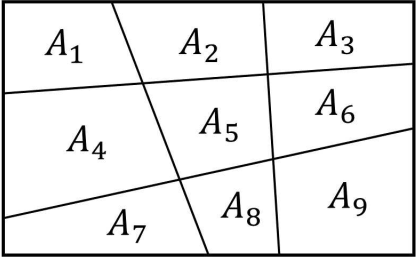
\includegraphics[width=10cm]{illustration_partition.png}
    \caption{Un domaine rectangulaire du plan est divisé en 9 sous-ensembles disjoints $A_1, A_2,..., A_9$ (extrait de \cite{3})}
    \label{fig7.1}
\end{figure} 

\vspace{2ex}
Les partitions seront représentées par des lettres grecques minuscules. On introduit la partition de points distincts qui nous servira dans la partie sur les partitions génératrices :

\begin{equation}
    \epsilon = \left\{\left\{x\right\} : x \in \Omega \right\}
\end{equation}

\vspace{2ex}
Soit $\alpha = \left\{A_1,..., A_{|\alpha|}\right\}=\left\{A_a : 1 \geq a \geq |\alpha|\right\}$ et $\beta = \left\{B_1,..., B_{|\beta|}\right\}=\left\{B_a : 1 \geq a \geq |\beta|\right\}$ des partitions de $\Omega$, où $|\alpha|$ désigne le cardinal de l'ensemble $\alpha$.

\vspace{2ex}
On défini la partition $\alpha \lor \beta = \left\{A_a \cap B_b : 1 \geq a \geq |\alpha|, 1 \geq b \geq |\beta|\right\}$ comme le raffinement de $\alpha$ et $\beta$. La raffinement de plus de deux partitions est défini de manière récursive.

\vspace{2ex}
L'entropie de $\alpha$ est définie par

\begin{equation}
    H_{\mu}(\alpha) = - \sum_{a=1}^{|\alpha|}\mu(A_a)log_{\mu}(A_a)
\end{equation}

où le logarithme peut être en base 2 ou e.

\vspace{2ex}
Si $X : \Omega \longrightarrow \left\{1,...,|\alpha|\right\}$ est une variable aléatoire définie par $X(\omega) = a$ si et seulement si $\omega \in A_a$, alors $H_\mu(\alpha)$ coïncide avec l'entropie de Shannon de $X$,

\begin{equation}
    H(X) = - \sum_{a=1}^{|\alpha|}Pr\left\{X=a\right\}logPr\left\{X=a\right\}
\end{equation}

puisque la probabilité que $X=a$ est $Pr\left\{X=a\right\}=\mu\left\{X^{-1}(a)\right\}=\mu(A_a)$.

Comme vu précédemment, $H(X)$ mesure l'incertitude des valeurs prises par la variable aléatoire $X$.

\subsection*{Système dynamique et entropie}

\vspace{2ex}
Une fois que les espaces de probabilité et les partitions ont été introduits, l'ingrédient restant est le concept de dynamique ou de passage du temps.
Considérons un espace probabilisé $(\Omega,\mathcal{B},\mu)$ comme défini précédemment ainsi qu'une application mesurable $f : \Omega \longrightarrow \Omega$, i.e., $f^{-1}(B) \in \mathcal{B}$ pour tout $B \in \mathcal{B}$. Le lien entre l'espace de probabilité et l'application mesurable réside dans le fait que $f$ préserve la mesure, i.e. $\mu(f^{-1}(B))=\mu(B)$ pour tout $B \in \mathcal{B}$. Alternativement, on dit que $f$ est $\mu$-invariant ou bien que la mesure $\mu$ est $f$-invariante. En particulier, si on prend une partition $\alpha =\left\{A_a : 1 \geq a \geq |\alpha|\right\}$ de $\Omega$, alors $f^{-1}(\alpha) =\left\{f^{-1}(A_a) : 1 \geq a \geq |\alpha|\right\}$ est aussi une partition de $\Omega$.
Si, de plus, $f$ est une application préservant la mesure, un à un, et que $f^{-1}$ préserve également la mesure, alors on dit que $f$ est une application inversible préservant la mesure.

\vspace{2ex}
En s'appuyant sur les définitions précédentes, on appelle $(\Omega, \mathcal{B}, \mu, f)$ un système dynamique (préservant la mesure). Les dynamiques de ce système sont générées par les itérations $f^{n+1}(x) = f(f^n(x))$ au pas de temps discrets $n \in \mathbb{T}$. La séquence $(f^n(x))_{n \in \mathbb{T}}$ est appelée orbite ou trajectoire avant (resp. complète) de $x$ si $\mathbb{T} = \mathbb{N}_0$ (resp. $\mathbb{T} = \mathbb{Z}$); $x$ est parfois appelé la condition initiale.

\vspace{2ex}
A ce stade et pour la suite, il nous faut introduire une définition. Il est dit que $(\Omega_1,\mathcal{B}_1,\mu_1,f_1)$ et $(\Omega_2,\mathcal{B}_2,\mu_2,f_2)$ sont isomorphes s'il existe $M_i \in \mathcal{B}_i (i=1,2)$ avec $\mu(M_i)=1$ et $f(M_i) \subset M_i$, et qu'il existe une application inversible préservant la mesure$\Phi: M_1 \longrightarrow M_2$ avec $(\Phi \circ f_1)(x)=(f_2 \circ \Phi)(x)$, $\forall x \in M-1$. L'application $\Phi$ est appelée un isomorphisme.

\vspace{2ex}
Si l'on considère le système dynamique à mesure preservée $(\Omega,\mathcal{B},\mu,f)$ et une partition $\alpha = \left\{A_a : 1 \geq a \geq |\alpha|\right\}$ de $(\Omega,\mathcal{B},\mu)$, alors  

\begin{equation}
    h_{\mu} = \lim_{n \to \infty} \frac{1}{n} H_{\mu}(\bigvee_{i=0}^{n-1} f^{-i}\alpha)
\end{equation}

Est appelée l'entropie de f par rapport à la partition $\alpha$. Avec l'équation (5.7), on obtient

\begin{equation}
    H_{\mu}(\bigvee_{i=0}^{n-1} f^{-i}\alpha) = \sum_{a_0,a_1,...,a_{n-1}} \mu(A_{a_0} \cap f^{-1}A_{a_1} \cap...\cap f^{-n+1}A_{a_{n-1}})log\mu(A_{a_0} \cap f^{-1}A_{a_1} \cap...\cap f^{-n+1}A_{a_{n-1}})
\end{equation}

On peut à présent introduire l'entropie de Kolmogorov-Sinai de l'application f avec le même système dynamique à mesure preservée que précédemment $(\Omega,\mathcal{B},\mu, f)$. Celle-ci est définie de la manière suivant

\begin{equation}
    h_{\mu}(f) = sup h_{\mu}(f,\alpha)
\end{equation}

où le supremum est pris sur toutes les partitions finies de $(\Omega,\mathcal{B},\mu)$.  On verra par la suite que le supremum est atteint pour des partitions génératrices dans l'espace des phases (états).

\subsection*{Dynamique symbolique par rapport à une partition}

\vspace{2ex}
On a vu que tout processus aléatoire stationnaire à temps discret sur un espace de probabilité correspond à un système dynamique préservant la mesure.

\vspace{2ex}
En effet, soit $Z = \left\{Z_n\right\}_{n \in \mathbb{T}}$ un processus aléatoire (i.e. stochastique) sur un espace de probabilité $(\Omega,\mathcal{B},\mu)$ avec comme états $\left\{1,...,k\right\}$ et une distribution jointe de probabilité $p(z_{n_1},...,z_{n_r})$ où $r \geq 1$ et $z_{n_1},...,z_{n_r} \in \left\{1,...,k\right\}$. On note $\left\{1,...,k\right\}\}^\mathbb{T}$ l'ensemble de toutes les séquences ayant comme symboles $\left\{1,...,k\right\}$. On définit l'application de codage mesurable $\Phi : \Omega \longrightarrow \left\{1,...,k\right\}$ tel que $\Phi(\omega) = (Z_n(\omega))_{n \in \mathbb{T}}$ et $\mathcal{C}$ la tribu produit générée par les ensembles cylindriques, i.e. les ensembles des séquences à valeurs dans $\left\{1,...,k\right\}^\mathbb{T}$ avec un nombre fini de composantes fixées. En outre, on dote l'espace mesurable $(\left\{1,...,k\right\}^\mathbb{T}, \mathcal{C})$ d'une mesure transportée $m = \mu \circ \Phi^{-1}$, i.e.,

\begin{equation}
    m(C) = \mu(\Phi^{-1}C), C \in \mathcal{C}
\end{equation}

de sorte à ce que $\Phi$ préserve la mesure. 

L'opérateur de décalage $\sigma : (z_n)_{n \in\mathbb{T}} \longrightarrow (z_{n+1})_{n \in \mathbb{T}}$ sur l'espace de probabilité $(\left\{1,...,k\right\}\}^\mathbb{T}, \mathcal{C},m)$ est alors $m$-invariant de par la stationarité de $Z$.
On a alors $(\left\{1,...,k\right\}\}^\mathbb{T}, \mathcal{C}, m, \sigma)$ qui constitue un système dynamique préservant la mesure que l'on appelle système dynamique discret ou support de $Z$, $Supp(Z)$.
Les états du système dynamique $Supp(Z)$ sont les trajectoires ou réalisations $(z_n)_{n \in \mathbb{T}}$ du processus aléatoire $\textbf{Z}$. Si $n=0$ correspond au temps actuel, les valeurs de $\textbf{Z}$ sont mis à jour grâce à l'application de décalage $\sigma$.

Comme vu dans les parties précédentes, le taux d'entropie de Shannon du processus stochastique stationnaire $\textbf{Z}=\left\{Z_n\right\}_{n\in\mathbb{T}}$, avec comme états $(\left\{1,...,k\right\}\}$, est défini par

\begin{equation}
    h(\textbf{Z})=-\lim_{n \to \infty}\sum_{z_1,...,z_n}Pr\left\{Z_1=z_1, ...,Z_n=z_n\right\}logPr\left\{Z_1=z_1, ...,Z_n=z_n\right\}
\end{equation}

Cette limite converge car le processus stochastique $\textbf{Z}$ est stationnaire. 

\vspace{2ex}
Nous venons de voir que tout processus aléatoire stationnaire peut être associé à un système dynamique appelé son support. Cette association est rendue possible par l'application de codage $\Phi$. Il se trouve que ce qui nous intéresse dans notre étude est le corrolaire : tout système dynamique peut être associé à un processus stochastique stationnaire avec un nombre d'états fini appelé dynamique symbolique. Cette seconde association est rendue possible par les partitions, c'est ce que l'on va expliciter par la suite.

\vspace{2ex}
On reprend le système dynamique à mesure preservée $(\Omega,\mathcal{B},\mu,f)$ et une partition $\alpha = \left\{A_a : 1 \geq a \geq |\alpha|\right\}$ de $(\Omega,\mathcal{B},\mu)$ introduit.e.s. On définit, pour tout $n \in \mathbb{T}$, l'application mesurable $Z_n^{\alpha}: \Omega \longrightarrow \left\{1,...,|\alpha|\right\}\}$ telle que

\begin{equation}
    Z_n^{\alpha}(x)=a_n \iff f^n(x)\in A_{a_n}
\end{equation}

Alors $\textbf{Z}^{\alpha}=\left\{Z_n^{\alpha}\right\}_{n\in\mathbb{T}}$ est un processus stochastique stationnaire. En effet, la distribution de probabilité jointe de $\textbf{Z}^{\alpha}$ nous est donnée par le biais de la mesure de probabilité $\mu$

\begin{equation}
    Pr \left\{ Z_0^{\alpha}=a_0, ...,Z_n^{\alpha}=a_n \right\} = \mu \left\{ x \in \Omega :x \in A_{a_0},f(x) \in A_{a_1},...,f^n(x) \in A_{a_n}\right\} = \mu\left\{A_{a_0} \cap f^{-1}A_{a_1} \cap...\cap f^{-n}A_{a_n}\right\}
\end{equation}

La stationnarité de $\textbf{Z}$ est triviale de par le fait que $\mu$ soit $f$-invariant.

\vspace{2ex}
La séquence $(a_n)_{n\in\mathbb{T}}$ constitue la trajectoire symbolique de $x$ par rapport à la partition $\alpha$, $a_n \in \left\{1,...,|\alpha|\right\}$ étant le nième symbole de la trajectoire.

\vspace{2ex}
$\textbf{Z}^{\alpha}=\left\{Z_n^{\alpha}\right\}_{n\in\mathbb{T}}$ défini dans l'équation (3.19) est la dynamique symbolique de $f$ par rapport à la partition $\alpha$. On en déduit de l'équation (3.20) que

\begin{equation}
    h(\textbf{Z}^{\alpha})=h_{\mu}(f,\alpha)
\end{equation}

C'est l'entropie de Kolmogorov-Sinai de l'application $f$ préservant la mesure $\mu$ par rapport à la partition $\alpha$ qui est égale à l'entropie de sa dynamique symbolique par rapport à la même partition. Cela prouve que $h_{\mu}(f,\alpha)$ existe toujours car $\mathbf{Z}^{\alpha}$ est un processus stochastique stationnaire.

\subsection*{Partitions génératrices}

Le point clef de la représentation symbolique est l'existence de partitions $\alpha$ de $(\Omega, \mathcal{B},\mu)$ telles que la correspondance entre les trajectoires $(f^n(x))_{n\in\mathbb{T}}$ d'une application qui préserve la mesure $f:\Omega\longrightarrow\Omega$ et leurs représentations symboliques $\Phi^{\alpha}=(a_n)_{n\in\mathbb{T}}$ soit exacte.

\vspace{2ex}
Une partition $\alpha$ de $(\Omega, \mathcal{B},\mu)$ est appelée partition génératrice unilatérale pour une application préservant la mesure $f : \Omega \longrightarrow \Omega$ si $\bigvee_{i=0}^{\infty}f^{-i}\alpha=\epsilon$. En outre, si de plus $f$ est inversible et $\bigvee_{i\in\mathbb{Z}}^{\infty}f^{-i}\alpha=\epsilon$ alors $\alpha$ est une partition génératrice bilatérale pour $f$.

\vspace{2ex}
Si $\alpha$ est une partition génératrice pour $f$, alors $Supp(\mathbf{Z}^{\alpha})$ est isomorphe à $(\Omega, \mathcal{B},\mu,f)$. Ce théorème implique la correspondance un à un des trajectoires des séries temporelles avec leurs représentations symboliques grâce aux partitions génératrices.

\vspace{2ex}
On considère toujours le même système dynamique à mesure préservée $(\Omega, \mathcal{B},\mu,f)$. Le théorème de Kolmogorov-Sinai nous dit que si $\alpha$ est une partition génératrice pour $f$, alors on a

\begin{equation}
    h_{\mu}(f)=h_{\mu}(f,\alpha)
\end{equation}

Enfin, les partitions génératrices nous permettent de faire le lien entre le taux d'entropie de Shannon (5.19) et l'entropie de Kolmogorov-Sinai via les dynamiques symboliques. En effet, si $\alpha$ est une partition génératrice pour $f$, alors on obtient à partir de l'équation (5.22) et en vertue du théorème (5.23)

\begin{equation}
    h(\mathbf{X}^{\alpha})=h_{\mu}(f)
\end{equation}

De plus, de par le fait que $(\Omega, \mathcal{B},\mu,f)$ et $Supp(\mathbf{Z}^{\alpha})=(\left\{1,...,|\alpha|\right\}^\mathbb{T}, \mathcal{C}, m, \sigma)$ soient isomorphes, l'équation (5.24) devient

\begin{equation}
    h(\mathbf{X}^{\alpha})=h_{\mu}(f)=h_m(\sigma)
\end{equation}
